\documentclass{beamer}
\usepackage{amsmath, amssymb}
\usepackage{graphicx}
\usepackage{listings}
\usepackage{color}
\usepackage{tcolorbox,fancyvrb,xcolor,tikz}
\tcbuselibrary{skins,breakable}

\setbeamertemplate{footline}[frame number]

\newenvironment{VerbatimIN}
 {\VerbatimEnvironment
  \begin{tcolorbox}[
    breakable,
    colback=lightgray,
    spartan
  ]%
  \begin{Verbatim}}
 {\end{Verbatim}\end{tcolorbox}}

 \newenvironment{VerbatimOUT}
 {\VerbatimEnvironment
  \begin{tcolorbox}[
    breakable,
    spartan
  ]%
  \begin{Verbatim}}
 {\end{Verbatim}\end{tcolorbox}}

\definecolor{darkred}{rgb}{0.75, 0, 0}
\definecolor{orange}{rgb}{1, 0.65, 0}
\definecolor{violet}{rgb}{0.58, 0, 0.83}
\definecolor{darkgray}{rgb}{0.33, 0.33, 0.33}
\definecolor{darkgreen}{rgb}{0.0, 0.5, 0.0}

\title{Mixed Effects Models - Day 5}
\subtitle{Theory of Mixed Effect Models}
\author{Marieke Wesselkamp \\ Department of Biometry and Environmental Systems Analysis \\
Albert-Ludwigs-University of Freiburg (Germany)}
\date{November 2024}

\begin{document}

\frame{\titlepage}


% Slide 2: Linear Effects Model
\begin{frame}{Linear Effects Model in general matrix notation}
\[
\mathbf{y} = \mathbf{X} \cdot \mathbf{b} + \mathbf{e}
\]
\[
\mathbf{e} \sim \mathcal{N}(0, \sigma^2_{\epsilon} \cdot \mathbf{I})
\]
where:
\begin{itemize}
  \item $\mathbf{y}$: measured response values
  \item $\mathbf{X}$: design matrix
  \item $\mathbf{b}$: parameter vector of the design matrix
  \item $\mathbf{e}$: error vector with $mean = 0$, $variance = \sigma^2_{\epsilon} \cdot \mathbf{I}$
  \item $\mathbf{\sigma^2_{\epsilon} \cdot \mathbf{I}}$: error or residual variance-covariance matrix
\end{itemize}
\vspace{0.5cm}

\pause

\textbf{From now on}: $\sigma^2_{\epsilon} \cdot \mathbf{I} = \mathbf{R}$ (Residual = R-side).

\end{frame}

% Slide 3: Linear Mixed Effects Model
\begin{frame}{Linear Mixed Effects Model in general matrix notation}
\[
\mathbf{y} = \mathbf{X} \cdot \mathbf{b} + \mathbf{Z} \cdot \mathbf{u} + \mathbf{e}
\]
\[
\mathbf{e} \sim \mathcal{N}(0, \mathbf{R}), \quad \mathbf{u} \sim \mathcal{N}(0, \mathbf{G}), \quad \mathbf{u} \bot \mathbf{e}
\]
where:
\begin{itemize}
  \item $\mathbf{X}$: Fixed Effects design matrix
  \item $\mathbf{b}$: Fixed Effects parameter vector
  \item $\mathbf{e}$: Error vector
  \item $\mathbf{R}$: Residual variance-covariance matrix (R-side)
  \pause
  \item $\mathbf{Z}$: Random Effects design matrix
  \item $\mathbf{u}$: Random Effects parameter vector
  \item $\mathbf{R}$: Random effects variance-covariance matrix (G-side)
\end{itemize}
\end{frame}

% Slide 5: Matrix Representation of Response
\begin{frame}[fragile]
\frametitle{Let's break it down}
    \large The response vector \textbf{y}
    \begin{columns}
        \begin{column}{0.5\textwidth}        
        \normalsize
            \[
            \mathbf{y} = \left( 
            \begin{array}{c} 
            \color{darkred}{y_1} \\ 
            \color{darkred}{y_2} \\ 
            \color{orange}{y_3} \\ 
            \color{orange}{y_4} \\ 
            \color{violet}{y_5} \\ 
            \color{violet}{y_6} \\ 
            \color{darkgray}{y_7} \\ 
            \color{darkgray}{y_8} 
            \end{array}\right) = \left( 
            \begin{array}{c} 
            \color{darkred}{1.63} \\ 
            \color{darkred}{8.03} \\ 
            \color{orange}{2.68} \\ 
            \color{orange}{0.47} \\ 
            \color{violet}{3.77} \\ 
            \color{violet}{3.76} \\ 
            \color{darkgray}{2.15} \\ 
            \color{darkgray}{5.61} 
            \end{array}\right)
            \]
        \end{column}
        \begin{column}{0.5\textwidth}
            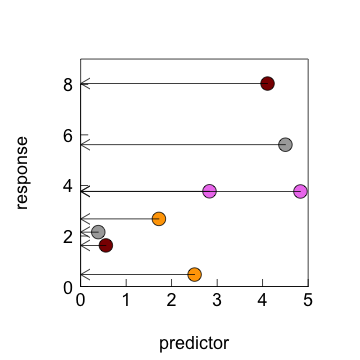
\includegraphics[width=\textwidth]{lectures/day_5_theory_of_mems/figures/unnamed-chunk-3-1.png}
        \end{column}
    \end{columns}
    \vspace{0.3cm}
    
    \large\textbf{4} groups are measured \textbf{2} times each...
\end{frame}

% Slide 6: Fixed Effects Design Matrix
\begin{frame}
\frametitle{Fixed Effects Design Matrix X}
\large ...at two different values per group of a continous predictor
\begin{columns}
        \begin{column}{0.5\textwidth}
            \[
\mathbf{X} = \left( 
\begin{array}{cc} 
\color{darkred}{1} & \color{darkred}{0.56} \\ 
\color{darkred}{1} & \color{darkred}{4.11} \\ 
\color{orange}{1} & \color{orange}{1.72} \\ 
\color{orange}{1} & \color{orange}{2.51} \\ 
\color{violet}{1} & \color{violet}{2.83} \\ 
\color{violet}{1} & \color{violet}{4.83} \\ 
\color{darkgray}{1} & \color{darkgray}{0.39} \\ 
\color{darkgray}{1} & \color{darkgray}{4.5} 
\end{array}\right)
\]
        \end{column}
        \begin{column}{0.5\textwidth}
            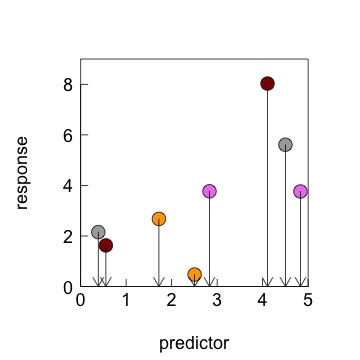
\includegraphics[width=\textwidth]{lectures/day_5_theory_of_mems/figures/unnamed-chunk-4-1.png}
        \end{column}
    \end{columns}

\end{frame}

\begin{frame}
\frametitle{The Parameter Vector b}
    \begin{columns}
        \begin{column}{0.5\textwidth}
\[
\boldsymbol{b} = 
\begin{pmatrix}
\beta_0 \\
\beta_1
\end{pmatrix} =
\begin{pmatrix}
intercept \\
slope
\end{pmatrix}
\]
\[
=
\begin{pmatrix}
0.98 \\
0.48
\end{pmatrix}
\]
        \end{column}
        \begin{column}{0.5\textwidth}
            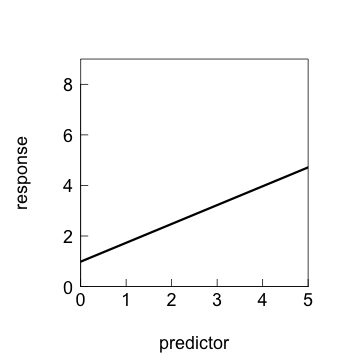
\includegraphics[width=\textwidth]{lectures/day_5_theory_of_mems/figures/unnamed-chunk-5-1.png}
        \end{column}
    \end{columns}
    \vspace{0.3cm}
    
    \large \textit{The parameter vector b describes the average deterministic part of the model}
\end{frame}

% Slide 7: Random Effects Design Matrix
\begin{frame}{Random Effects Design Matrix Z}
\begin{columns}
        \begin{column}{0.5\textwidth}
\[
\mathbf{Z} = \left( 
\begin{array}{cccc} 
\color{darkred}{1} & . & . & . \\ 
\color{darkred}{1} & . & . & . \\ 
. & \color{orange}{1} & . & . \\ 
. & \color{orange}{1} & . & . \\ 
. & . & \color{violet}{1} & . \\ 
. & . & \color{violet}{1} & . \\ 
. & . & . & \color{darkgray}{1} \\ 
. & . & . & \color{darkgray}{1} 
\end{array}\right)
\]
        \end{column}
        \begin{column}{0.5\textwidth}
        \large
            1) There are only 1s because it is a \textbf{Random Intercept} model \\
            \vspace{0.3cm}
            
            2) It is \textbf{sparse} = empty elements because of the grouping
        \end{column}
    \end{columns}

\end{frame}

% Slide 8: Random Effects Parameter Vector
\begin{frame}{Random Effects Parameter Vector u}
\large \textbf{u} values as group-specific \textbf{deviations} from the population average intecept $\beta_0$
\begin{columns}
        \begin{column}{0.5\textwidth}
\[
\mathbf{u} = \left( 
\begin{array}{c} 
\color{darkred}{u_1} \\ 
\color{orange}{u_2} \\ 
\color{violet}{u_3} \\ 
\color{darkgray}{u_4} 
\end{array}\right) = \left( 
\begin{array}{c} 
\color{darkred}{0.24} \\ 
\color{orange}{-0.20} \\ 
\color{violet}{-0.12} \\ 
\color{darkgray}{0.09} 
\end{array}\right)
\]
        \end{column}
        \begin{column}{0.5\textwidth}
            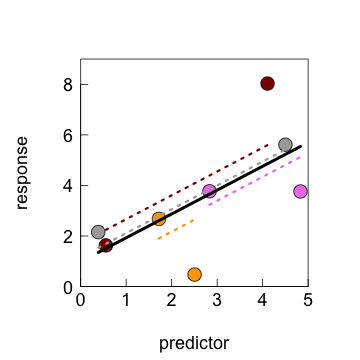
\includegraphics[width=\textwidth]{lectures/day_5_theory_of_mems/figures/unnamed-chunk-6-1.png}
        \end{column}
    \end{columns}
    \vspace{0.2cm}
\large\textit{The random intercepts shift the group-specific lines up or down}
\end{frame}

% Slide 10: Error Vector
\begin{frame}{Error Vector $\epsilon$}
    \begin{columns}
        \begin{column}{0.5\textwidth}
\[
\mathbf{e} = \left( 
\begin{array}{c} 
\color{darkred}{\epsilon_1} \\ 
\color{darkred}{\epsilon_2} \\ 
\color{orange}{\epsilon_3} \\ 
\color{orange}{\epsilon_4} \\ 
\color{violet}{\epsilon_5} \\ 
\color{violet}{\epsilon_6} \\ 
\color{darkgray}{\epsilon_7} \\ 
\color{darkgray}{\epsilon_8} 
\end{array}\right) = \left( 
\begin{array}{c} 
\color{darkred}{-0.12} \\ 
\color{darkred}{2.93} \\ 
\color{orange}{0.27} \\ 
\color{orange}{-2.67} \\ 
\color{violet}{0.23} \\ 
\color{violet}{-1.67} \\ 
\color{darkgray}{0.72} \\ 
\color{darkgray}{0.30} 
\end{array}\right)
\]
        \end{column}
        \begin{column}{0.5\textwidth}
            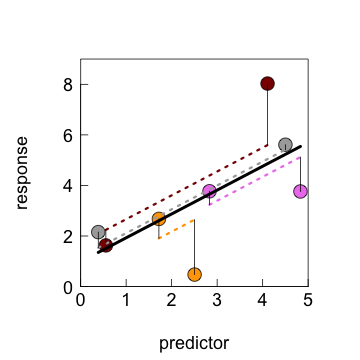
\includegraphics[width=\textwidth]{lectures/day_5_theory_of_mems/figures/unnamed-chunk-7-1.png}
        \end{column}
    \end{columns}
    \vspace{0.3cm}
    
\large \textit{Deviations of the measurements from the random effects values u = the deviations from the deviations}
\end{frame}

% Slide 11: Two Stochastic Parts
\begin{frame}{}
\Large
\underline{A Mixed Effects Model has two stochastic parts:}
\vspace{0.2cm}

The \textbf{first stochastic part} $\mathbf{u} \sim \mathcal{N}(0, \mathbf{G})$ is describing how the random effects $\mathbf{u}$ vary around $0$ and is given by the random effects variance-covariance matrix $\mathbf{G}$\footnote{This is now the third variance - covariance matrix we encounter after the ones for the model parameters and the residual errors.}.

\end{frame}

% \begin{frame}{Two Stochastic Parts in Mixed Models}
% \Large
% A Mixed Effects Model has two stochastic parts:
% \vspace{0.2cm}

% \begin{enumerate}
%   \item $\mathbf{u} \sim \mathcal{N}(0, \mathbf{G})$ describing how the random effects $\mathbf{u}$ vary around $0$ and is given by the random effects variance-covariance matrix $\mathbf{G}$.
%   \item $\mathbf{e} \sim \mathcal{N}(0, \mathbf{R})$ describes how the residuals vary after accounting for fixed and random effects.
% \end{enumerate}
% \end{frame}

% Slide 12: Random Intercept Model Variance
\begin{frame}{Random Intercept Model Variance}
\Large
In the simplest case of a Random Intercept Model, $\mathbf{G}$ has only one value for the variance of random intercepts (\textbf{u}) among groups:
\[
\mathbf{G} = \left( \mathit{d}^2 \right) = 0.29
\]
\end{frame}

\begin{frame}
\frametitle{}
\Large
The assumption is, that each group is independently measured of each other, i.e. the random effect $\mathit{u_i}$ of group $\mathit{g_i}$ has nothing to do with other groups.
\vspace{0.3cm}

\noindent\fbox{
    \parbox{\textwidth}{
        \textit{This is \textbf{NOT} the case anymore if there are    \textbf{multiple} Random Effects in a data set. In this case, one has to account for a more complex Random Effects Structure to make $\mathbf{u_i}$ independent = nested or crossed Random Effects}
    }
}
\end{frame}

\begin{frame}{}
\Large
\underline{A Mixed Effects Model has two stochastic parts:}
\vspace{0.2cm}

The \textbf{second stochastic part} is the remaining and unexplained (residual) variance $\mathbf{e} \sim \mathcal{N}(0, \mathbf{R})$

It describes how the measurements $\mathbf{e}$ \textbf{AFTER} accounting for the fixed and the random effects vary around 0 and is given by the residual variance - covariance matrix \textbf{R}.\footnote{That sounds suspiciously like the Linear Model, where the resulting off-diagonal zeros say that errors are independent}
\vspace{0.2cm}

In it's simplest form: $\mathbf{R} = \sigma^2 \mathbf{I}$ 
\end{frame}

\begin{frame}
\frametitle{}
\centering
\Large \textit{Indeed, there are \textbf{zero} off-diagonals}

\[
\mathbf{R} = \left( 
\begin{array}{cccccccc} 
\color{darkred}{\sigma^2} & \color{darkred}{0} & . & . & . & . & . & .\\ 
\color{darkred}{0} & \color{darkred}{\sigma^2} & . & . & . & . & . & .\\ 
. & . & \color{orange}{\sigma^2} & \color{orange}{0} & . & . & . & .\\ 
. & . & \color{orange}{0} & \color{orange}{\sigma^2} & . & . & . & .\\ 
. & . & . & . & \color{violet}{\sigma^2} & \color{violet}{0} & . & .\\ 
. & . & . & . & \color{violet}{0} & \color{violet}{\sigma^2} & . & .\\ 
. & . & . & . & . & . & \color{darkgray}{\sigma^2} & \color{darkgray}{0}\\ 
. & . & . & . & . & . & \color{darkgray}{0} & \color{darkgray}{\sigma^2}
\end{array}\right)
\]
\end{frame}

% Slide 13: Combined Variance-Covariance Matrix $\mathbf{V}$
\begin{frame}{Combined Variance-Covariance Matrix $\mathbf{V}$}
\Large
The two stochastic parts combined in the variance-covariance matrix $\mathbf{V}$:
\[
\mathbf{V} = \mathbf{Z} \cdot \mathbf{G} \cdot \mathbf{Z}^T + \mathbf{R}
\]
\vspace{0.3cm}

\normalsize\textit{Can you see, that we are back to the linear model, if G = 0?}
\end{frame}

% Slide 14: Example of $\mathbf{V}$ Matrix
\begin{frame}{Example of $\mathbf{V}$ Matrix}
\large
The $\mathbf{V}$ matrix, where $\mathit{d^2}$ is the covariance of two values in a group:
\tiny
\[
\mathbf{V} = \left( 
\begin{array}{cccccccc} 
\color{darkred}{\sigma^2 + d^2} & \color{darkred}{d^2} & . & . & . & . & . & . \\ 
\color{darkred}{d^2} & \color{darkred}{\sigma^2 + d^2} & . & . & . & . & . & . \\
. & . & \color{orange}{\sigma^2 + d^2} & \color{orange}{d^2} & . & . & . & .\\ 
. & . & \color{orange}{d^2} & \color{orange}{\sigma^2 + d^2} & . & . & . & .\\ 
. & . & . & . & \color{violet}{\sigma^2 + d^2} & \color{violet}{d^2} & . & .\\ 
. & . & . & . & \color{violet}{d^2} & \color{violet}{\sigma^2 + d^2} & . & .\\ 
. & . & . & . & . & . & \color{darkgray}{\sigma^2 + d^2} & \color{darkgray}{d^2}\\ 
. & . & . & . & . & . & \color{darkgray}{d^2} & \color{darkgray}{\sigma^2 + d^2}
\end{array} \right)
\]
\large
$\mathbf{V}$ encodes the \textbf{independence of random effects} assumption, the \textbf{identical variance} assumption for residuals and random effects, and the \textbf{independence of errors} assumption.
\end{frame}

% Slide 15: Summary of Assumptions of LMM
\begin{frame}{Assumptions of Linear Mixed Models}
\[
\mathbf{y} = \mathbf{X} \cdot \mathbf{b} + \mathbf{Z} \cdot \mathbf{u} + \mathbf{e}
\]
\[
\mathbf{e} \sim \mathcal{N}(0, \mathbf{R}), \quad \mathbf{u} \sim \mathcal{N}(0, \mathbf{G}), \quad \mathbf{u} \bot \mathbf{e}
\]
Key assumptions:
\begin{itemize}
  \item $\mathbf{b}$ describes the deterministic trend averaged over the random effects $\mathbf{u}$.
  \item $\mathbf{u}$ are normally and independently distributed with mean 0 and variance $\mathbf{G}$.
  \item Residual errors $\mathbf{e}$ are normally and independently distributed within a group with mean 0 variance $\mathbf{R}$.
  \item $\mathbf{u}$ and $\mathbf{e}$ are independent of each other: among groups, there are no correlations of errors
  \item The variances and covariance do not depend on group: they all have the same values in each group
\end{itemize}
\end{frame}

\begin{frame}
\Large
\centering
So, that's the random \textbf{intercept} model...

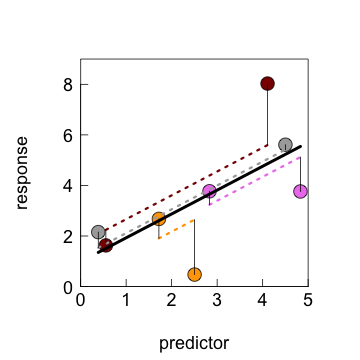
\includegraphics[width=0.7\textwidth]{lectures/day_5_theory_of_mems/figures/unnamed-chunk-8-1.png}
\end{frame}

\begin{frame}
\frametitle{A Random Intercept - Random Slope Model}

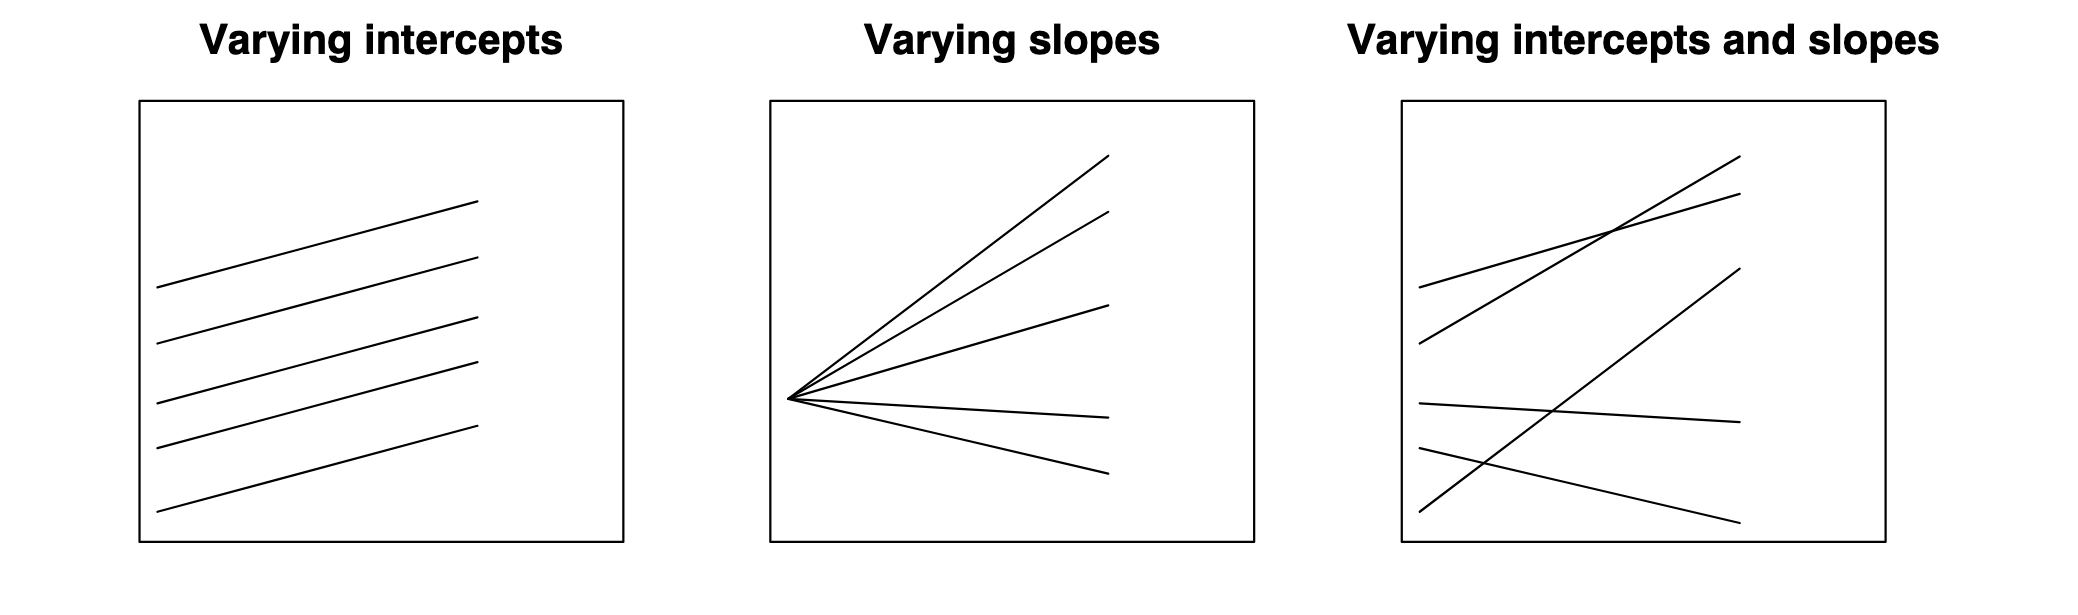
\includegraphics[width=0.9\textwidth]{lectures/day_5_theory_of_mems/figures/gelman_hill.png}

\Large
Two things change when going from a Random Intercept model to one that has also Random Slopes.
\end{frame}

\begin{frame}
\textbf{First}, the Random Effects design matrix $\mathbf{Z}$ has now a column that contains the values of the continous predictor to which each group respond in their own idiosyncratic way:
    \begin{columns}
        \begin{column}{0.55\textwidth}
        \small
\[
\mathbf{Z} = \left( 
\begin{array}{cccccccc} 
\color{darkred}{1} & \color{darkred}{x_1} & . & . & . & . & . & .\\ 
\color{darkred}{1} & \color{darkred}{x_2} & . & . & . & . & . & .\\ 
. & . & \color{orange}{1} & \color{orange}{x_3} & . & . & . & .\\ 
. & . & \color{orange}{1} & \color{orange}{x_4} & . & . & . & .\\ 
. & . & . & . & \color{violet}{1} & \color{violet}{x_5} & . & .\\ 
. & . & . & . & \color{violet}{1} & \color{violet}{x_6} & . & .\\ 
. & . & . & . & . & . & \color{darkgray}{1} & \color{darkgray}{x_7}\\ 
. & . & . & . & . & . & \color{darkgray}{1} & \color{darkgray}{x_8}
\end{array}\right)
\]
        \end{column}
        \begin{column}{0.45\textwidth}
            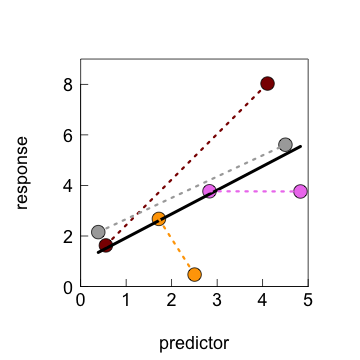
\includegraphics[width=\textwidth]{lectures/day_5_theory_of_mems/figures/unnamed-chunk-9-1.png}
        \end{column}
    \end{columns}
\end{frame}

\begin{frame}
\textbf{Second}, the Random Effects parameter vector $\mathbf{u}$ has now four values for the slope of these group-specific relationships:
    \begin{columns}
        \begin{column}{0.55\textwidth}
        \small
\[
\mathbf{u} = \left( 
\begin{array}{cc} 
\color{darkred}{u_1} & \color{darkred}{s_1} \\
\color{orange}{u_1} & \color{orange}{s_1} \\
\color{violet}{u_1} & \color{violet}{s_1} \\
\color{darkgray}{u_1} & \color{darkgray}{s_1} \\
\end{array}\right)
\]
        \end{column}
        \begin{column}{0.45\textwidth}
            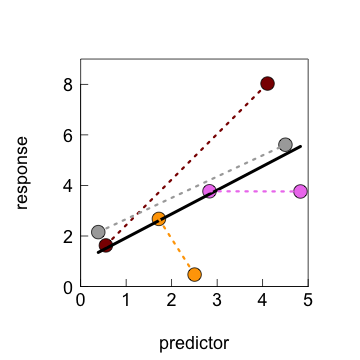
\includegraphics[width=\textwidth]{lectures/day_5_theory_of_mems/figures/unnamed-chunk-10-1.png}
        \end{column}
    \end{columns}

Which are group-specific deviations from the population average slope $\beta_1$ in addition to the deviations from the average intercept $\beta_0$
\end{frame}

\begin{frame}
\frametitle{}
Accordingly, the Random Effects Variance - Covariance matrix $\mathbf{G}$ has now four elements:
\[
\begin{pmatrix}
\mathit{u_i} \\
\mathit{s_i}
\end{pmatrix}
\sim \mathcal{N}(0, \mathbf{G})
\]
where
\[
\mathbf{G} = 
\begin{pmatrix}
\mathit{d_{11}}^2 \hspace{0.2cm} \mathit{d_{12}}^2 \\
\mathit{d_{21}}^2 \hspace{0.2cm} \mathit{d_{22}}^2
\end{pmatrix}
\]
\vspace{0.2cm}

$\mathit{d_{11}}^2$ is still the variance around the random intercepts, while $\mathit{d_{22}}^2$ is the variance around the random slopes among groups. $\mathit{d_{12}}^2 = \mathit{d_{21}}^2$ is the correlation between the random intercepts and slope.
\end{frame}

\begin{frame}
\large
\begin{itemize}
    \item Only a categorical variable can be a Random Effect (i.e.~a random intercept, equally used!). \textbf{Mostly, we do not fit a random slope without a random intercept}.
    \item A random slope can be categorical or continuous. The categorical random slope is sometimes called “random contrast”. It requires that each group has received each treatment. 
\end{itemize}
\end{frame}


\begin{frame}
\frametitle{Categorical random slope (Random contrast)}

Think about it as an \textbf{interaction} between two categorical variables.
\vspace{0.3cm}

    \begin{columns}
        \begin{column}{0.5\textwidth}
            Each group (red-blue) appears in each treatment (A-B)
                        
            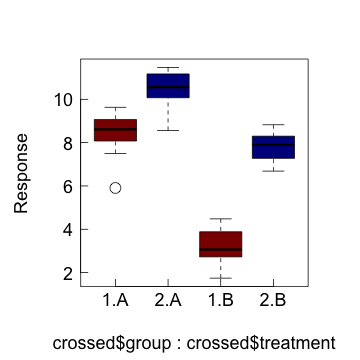
\includegraphics[width=\textwidth]{lectures/day_5_theory_of_mems/figures/unnamed-chunk-12-1.png}
        \end{column}
        \begin{column}{0.5\textwidth}
            Each group (red, darkred, blue and darkblue) appears \textbf{ONLY} in one of two treatments (reds-blues)
            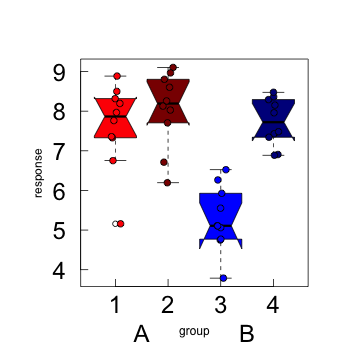
\includegraphics[width=\textwidth]{lectures/day_5_theory_of_mems/figures/unnamed-chunk-16-1.png}
        \end{column}
    \end{columns}
\end{frame}

\begin{frame}
\centering
\large
Random "contrast" design matrix
\vspace{0.2cm}

\[
\mathbf{Z} = \left( 
\begin{array}{cccccccc} 
\color{darkred}{1} & \color{darkred}{0} & . & . & . & . & . & .\\ 
\color{darkred}{1} & \color{darkred}{1} & . & . & . & . & . & .\\ 
. & . & \color{orange}{1} & \color{orange}{0} & . & . & . & .\\ 
. & . & \color{orange}{1} & \color{orange}{1} & . & . & . & .\\ 
. & . & . & . & \color{violet}{1} & \color{violet}{0} & . & .\\ 
. & . & . & . & \color{violet}{1} & \color{violet}{1} & . & .\\ 
. & . & . & . & . & . & \color{darkgray}{1} & \color{darkgray}{0}\\ 
. & . & . & . & . & . & \color{darkgray}{1} & \color{darkgray}{1}
\end{array}\right)
\]
\vspace{0.2cm}

\textit{We are not going to write out \textbf{V} with random slopes or contrasts. Derive this yourself by plugging the components into the equation on page 15.}
\end{frame}

\begin{frame}
    \centering\Huge\color{purple}{\textbf{Break!}}
\end{frame}

\begin{frame}{Multiple Random Effects}
    \Large
    The concept of \textbf{nested} versus \textbf{crossed} random effects occurs when you have two or more random effects in a dataset (multiple random effects).\\
    = Two or more \textbf{grouping} levels.

    \textit{In R-practice, we will have to specify if the random effects structure is random or crossed.}
\end{frame}

% Slide 2
\begin{frame}{Nested Random Effects - Beetles Example}
    \large
    \centering
    Populations are \emph{nested} in regions.

    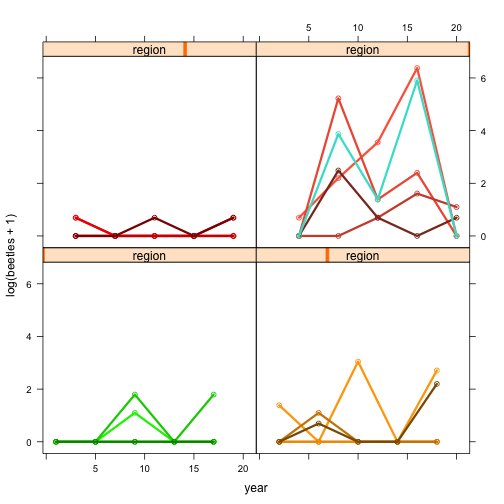
\includegraphics[width=0.6\textwidth]{lectures/day_5_theory_of_mems/figures/unnamed-chunk-17-1.png}
\end{frame}

% Slide 3
\begin{frame}{General mathematical formulation}
    \large
    \[
    \mathbf{y} = \mathbf{X} \cdot \mathbf{b} + \mathbf{Z_1} \cdot \mathbf{u_1} + \mathbf{Z_2} \cdot \mathbf{u_2} + \mathbf{e}
    \]
    \[
    \mathbf{e} \sim \mathcal{N}(0, \mathbf{R}), \quad \mathbf{u_1} \sim \mathcal{N}(0, \mathbf{G_1}), \quad \mathbf{u_2} \sim \mathcal{N}(0, \mathbf{G_2}), \quad \mathbf{u_{1,2}} \; \bot \; \mathbf{e}
    \]
\end{frame}

% Slide 4 - Nested Random Effects Visualization
\begin{frame}
    \Large
    This is \textbf{nested}: each tree is unique to each region. 
    \vspace{0.2cm}
    
    \begin{center}
        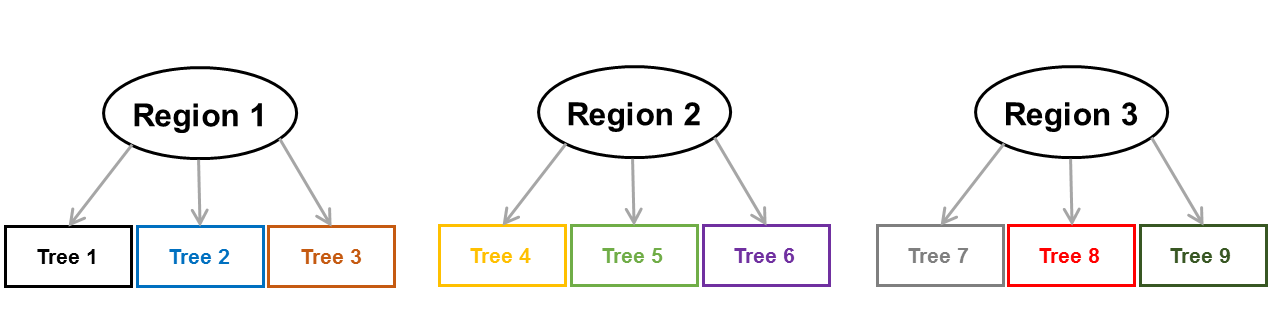
\includegraphics[width=\textwidth]{lectures/day_5_theory_of_mems/figures/two_RE_nested.png}
    \end{center}
    \vspace{0.2cm}

    \textit{Tree 1, for instance, has not been planted in Region 2, etc.}
\end{frame}

\begin{frame}
    \Large
    Here, you have that (imaginary) case! A \textbf{crossed} random effects structure:
    \vspace{0.2cm}
    
    \begin{center}
        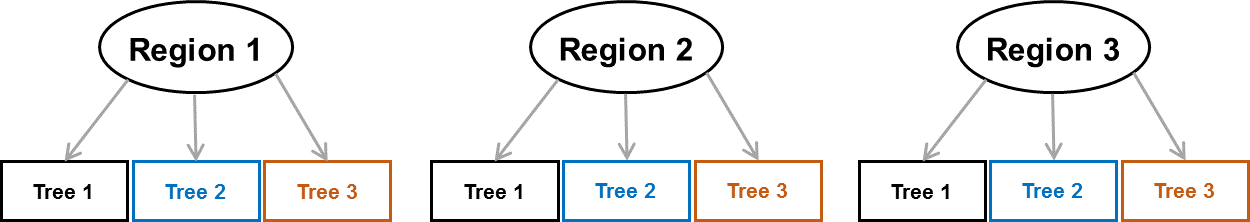
\includegraphics[width=\textwidth]{lectures/day_5_theory_of_mems/figures/Crossed_ind.trees.png}
    \end{center}
    \vspace{0.2cm}

    \textit{Does this setup make sense? ...Possibly in a transplantation experiment?}
\end{frame}

\begin{frame}
    \Large
    Another (more meaningful) \textbf{crossed} random effects structure:
    \vspace{0.2cm}
    
    \begin{center}
        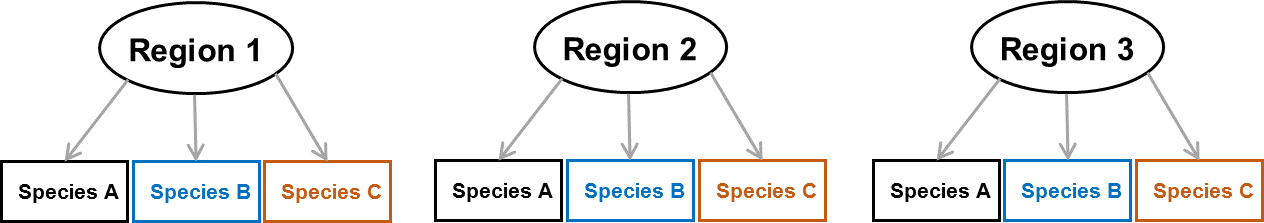
\includegraphics[width=\textwidth]{lectures/day_5_theory_of_mems/figures/two_RE_crossed.png}
    \end{center}
    \vspace{0.2cm}

    \textit{Individuals of each species appear in each region}
\end{frame}

\begin{frame}
    \Large
    \textbf{Erroneous} crossed Random effects:
    \vspace{0.2cm}
    
    \begin{center}
        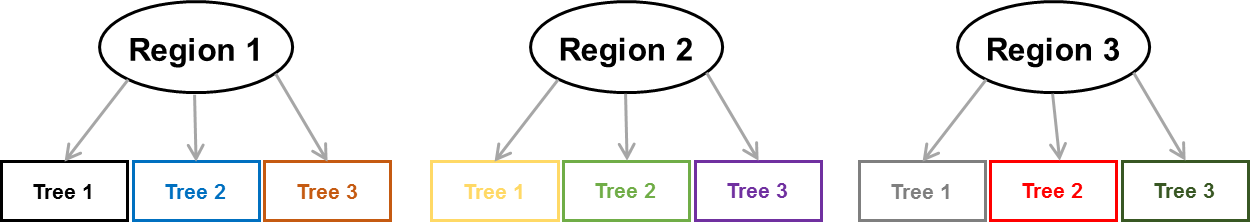
\includegraphics[width=\textwidth]{lectures/day_5_theory_of_mems/figures/ambigous_2.png}
    \end{center}
    \vspace{0.2cm}

    \textit{Different trees (colours!) are named identically across regions!}
    \vspace{0.2cm}
    
    \textbf{Beware the labeling of grouping variable levels!}
\end{frame}

\begin{frame}
    \Large
    More on crossed and nested effects \color{blue}\href{https://stats.stackexchange.com/questions/228800/crossed-vs-nested-random-effects-how-do-they-differ-and-how-are-they-specified}{here}
\end{frame}

% Slide 6 - REML Explanation
\begin{frame}{REML - Restricted Maximum Likelihood}
    \Large
    Fitting Mixed Effects Models and finding their parameters is somewhat different from Linear Models because by default, Mixed Effects Models use \textbf{Restricted Maximum Likelihood} (REML)
\end{frame}


\begin{frame}{Mixed Effects Model: Another Formulation}

\large
    \[
    \mathbf{y} = \mathbf{X} \cdot \mathbf{b} + \mathbf{Z} \cdot \mathbf{u} + \mathbf{e}
    \]
    \[
    \mathbf{e} \sim \mathcal{N}(0, \mathbf{R}), \quad \mathbf{u} \sim \mathcal{N}(0, \mathbf{G}), \quad \mathbf{u} \; \bot \; \mathbf{e}
    \]
    
\large
    The above mixed effect model could equivalently be written in this way:
    \vspace{0.2cm}
    
    \[
    \mathbf{y} = \mathcal{N} (\mathbf{X} \cdot \mathbf{b}, \mathbf{V})
    \]
    with the combined variance-covariance matrix
    \[
    \mathbf{V} = \mathbf{Z} \cdot \mathbf{G} \cdot \mathbf{Z^T} + \mathbf{R}
    \]
    where the GLS estimator for \textbf{b} was
    \[
    \mathbf{b} = ( \mathbf{X^T} \cdot \mathbf{V^{-1}} \cdot \mathbf{X}) \cdot \mathbf{X^T} \cdot \mathbf{V^{-1}} \cdot \mathbf{y}
    \]
\end{frame}

% Slide 8 - Optimisation Steps
\begin{frame}{Optimisation with REML}
During optimization, various steps are repeated:
    \vspace{0.2cm}
    
    \begin{enumerate}
        \item[Step 1:] Choose initial values for elements in $\mathbf{G}$ and $\mathbf{R}$
        \item[Step 2:] Calculate the covariance matrix $\mathbf{V}$ using these values
        \item[Step 3:] Calculate fixed effects parameter values $\mathbf{b}$ using $\mathbf{V}$
        \item[Step 4:] Update $\mathbf{V}$ using the newly calculated values $\mathbf{b}$ and thus changed $\mathbf{G}$ and $\mathbf{R}$
        \item[Step 5:] Check if likelihood has changed less than a certain degree (convergence criterion), if not, start again at Step 2 and repeat until convergence is attained
    \end{enumerate}
\end{frame}

\begin{frame}
    \frametitle{Convergence of MME's}
    \large
    A Mixed Effects Model is said to have converged if the fit is not becoming better with further iteration, i.e. when the likelihood doesn't change much when new parameters values are calculated
\end{frame}

\begin{frame}
\frametitle{Get random effects parameters}
    \large
    Finally, the random effects parameters \textbf{u} are calculated using the estimated values \textbf{b} and \textbf{V} and the data \textbf{y}
    \vspace{0.2cm}

    \[
    \mathbf{u} = \mathbf{G} \cdot \mathbf{Z^T} \mathbf{V^{-1}} \cdot (\mathbf{y} - \mathbf{X} \cdot \mathbf{b})
    \]
    \vspace{0.2cm}

    \textit{We estimate \textbf{b} and the components of \textbf{V}, but the Random Effects values are calculated.}
\end{frame}

\begin{frame}
\large
But the fixed effects parameters and the variance components are \textbf{estimated} and that estimation has an uncertainty:
\vspace{0.2cm}

However, in the iterative procedure above, it is assumed that the needed values in each step are known.
\vspace{0.2cm}

The uncertainty is thus not carried over, and estimates are \textbf{biased} if not corrected.
\end{frame}

\begin{frame}
\frametitle{ML: Biased variance estimate}
\large
The OLS estimate for the variance obtained by linear regression is unbiased, i.e. $\mathit{E}[\hat{\sigma}] = \sigma$: \\
Divided by \textbf{N-number of parameters}
\[
\sigma^2 = \frac{1}{N - p} \sum_{i=1}^{N} (y_i - \mu)^2
\]
\vspace{0.2cm}

The ML estimate is biased, i.e. $\mathit{E}[\hat{\sigma}] \neq \sigma$: \\
Doesn't account for model parameters
\[
\sigma^2 = \frac{1}{N} \sum_{i=1}^{N} (y_i - \mu)^2
\]
\end{frame}

\begin{frame}
\frametitle{REML: Unbiased variance estimate}
\large
With REML $\mathbf{y} = \mathcal{N} (\mathbf{X} \cdot \mathbf{b}, \mathbf{V})$ is transformed with a special (= orthogonal to \textbf{X}) matrix \textbf{A} to $\mathbf{A^T} \cdot \mathbf{y} = \mathcal{N} (\mathbf{0}, \mathbf{A^T} \cdot \mathbf{V} \cdot \mathbf{A})$ so that the ($\mathbf{X} \cdot \mathbf{b}$)
 part disappears.
 \vspace{0.2cm}

 \textit{No b coefficients to estimate, the variance components are now \textbf{unbiased} but the fixed effects are not anymore: important later for model inference and comparison}
\end{frame}

\begin{frame}
    \frametitle{Among- and within-group variance}
    \centering
    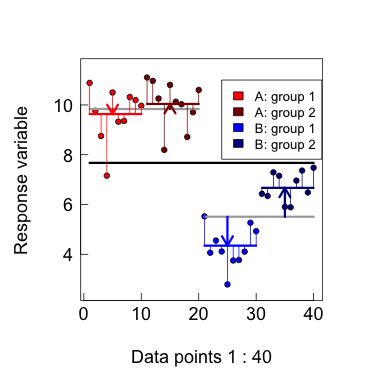
\includegraphics[width=0.7\textwidth]{lectures/day_5_theory_of_mems/figures/unnamed-chunk-20-1.png}
\end{frame}

\begin{frame}[fragile]
\textbf{With REML}, variance components (the random effects) are \textbf{larger}
\scriptsize
\begin{VerbatimIN}[numbers=left,numbersep=6pt]
VarCorr(m.reml.1)
\end{VerbatimIN}
\begin{VerbatimOUT}[numbers=left,numbersep=6pt]
Groups   Name        Std.Dev. Corr 
Subject  (Intercept) 24.7407       
         Days         5.9221  0.066
Residual             25.5918  
\end{VerbatimOUT}
\begin{VerbatimIN}[numbers=left,numbersep=6pt]
VarCorr(m.ml.1)
\end{VerbatimIN}
\begin{VerbatimOUT}[numbers=left,numbersep=6pt]
Groups   Name        Std.Dev. Corr 
Subject  (Intercept) 23.7798       
         Days         5.7168  0.081
Residual             25.5919       
\end{VerbatimOUT}
\end{frame}

\begin{frame}
\frametitle{Consequently:}

\Large
When comparing Mixed Effects Models that differ in their \textbf{random effects structure}, use REML
\vspace{0.2cm}

\textit{But because REML does its little trick on the \textbf{b}}
\vspace{0.2cm}

Use standard ML, when comparing Mixed Effects Models that differ in their \textbf{fixed effects structure}
\end{frame}

% Slide 18: Best Linear Unbiased Predictors (BLUPs)
\begin{frame}{Best Linear Unbiased Predictors (BLUPs)}
\large
Back to the Random Effects parameters \textbf{u} which give the deviation from the overall deterministic trend in the data:
\[
\mathbf{u} = \mathbf{G} \cdot \mathbf{Z}^T \mathbf{V}^{-1} (\mathbf{y} - \mathbf{X} \cdot \mathbf{b})
\]
When \textbf{u} are added to the expected values given by $\mathbf{X} \cdot \mathbf{b}$ one gets the so called \textbf{BLUPs} for best linear unbiased predictors.
\vspace{0.3cm}
\[
\mathbf{BLUPs} := \mathbf{X} \cdot \mathbf{b} + \mathbf{u}
\]
\vspace{0.3cm}
\textit{We will see all of this in practice}
\end{frame}

\begin{frame}{}
\large
BLUPs are...
\vspace{0.2cm}

    \begin{itemize}
        \item ...“linear” because they are a linear combination of $\mathbf{X} \cdot \mathbf{b}$ and \textbf{u}
        \item ...“unbiased” because their average equals the true expected group-specific trend
        \item ...“best” because they have the smallest variance of all linear predictors for the group-specific trend
    \end{itemize}
\end{frame}

\begin{frame}
    \huge
    \textbf{A demonstration of the effect of random effects at the example of the sleep deprivation study}
    \vspace{0.3cm}

    \normalsize
    Code and idea from Tristan Mahr and Douglas Bates \color{blue}\href{https://www.tjmahr.com/plotting-partial-pooling-in-mixed-effects-models/}{here}
\end{frame}

\begin{frame}
\begin{itemize}
    \item Seperate analysis for each person: \textbf{no pooling}; e.g. by adding 'person' as a covariate in a Linear Model
    \item Ignoring the data grouping in a Linear Model \textbf{complete pooling}
\end{itemize}
    \centering
    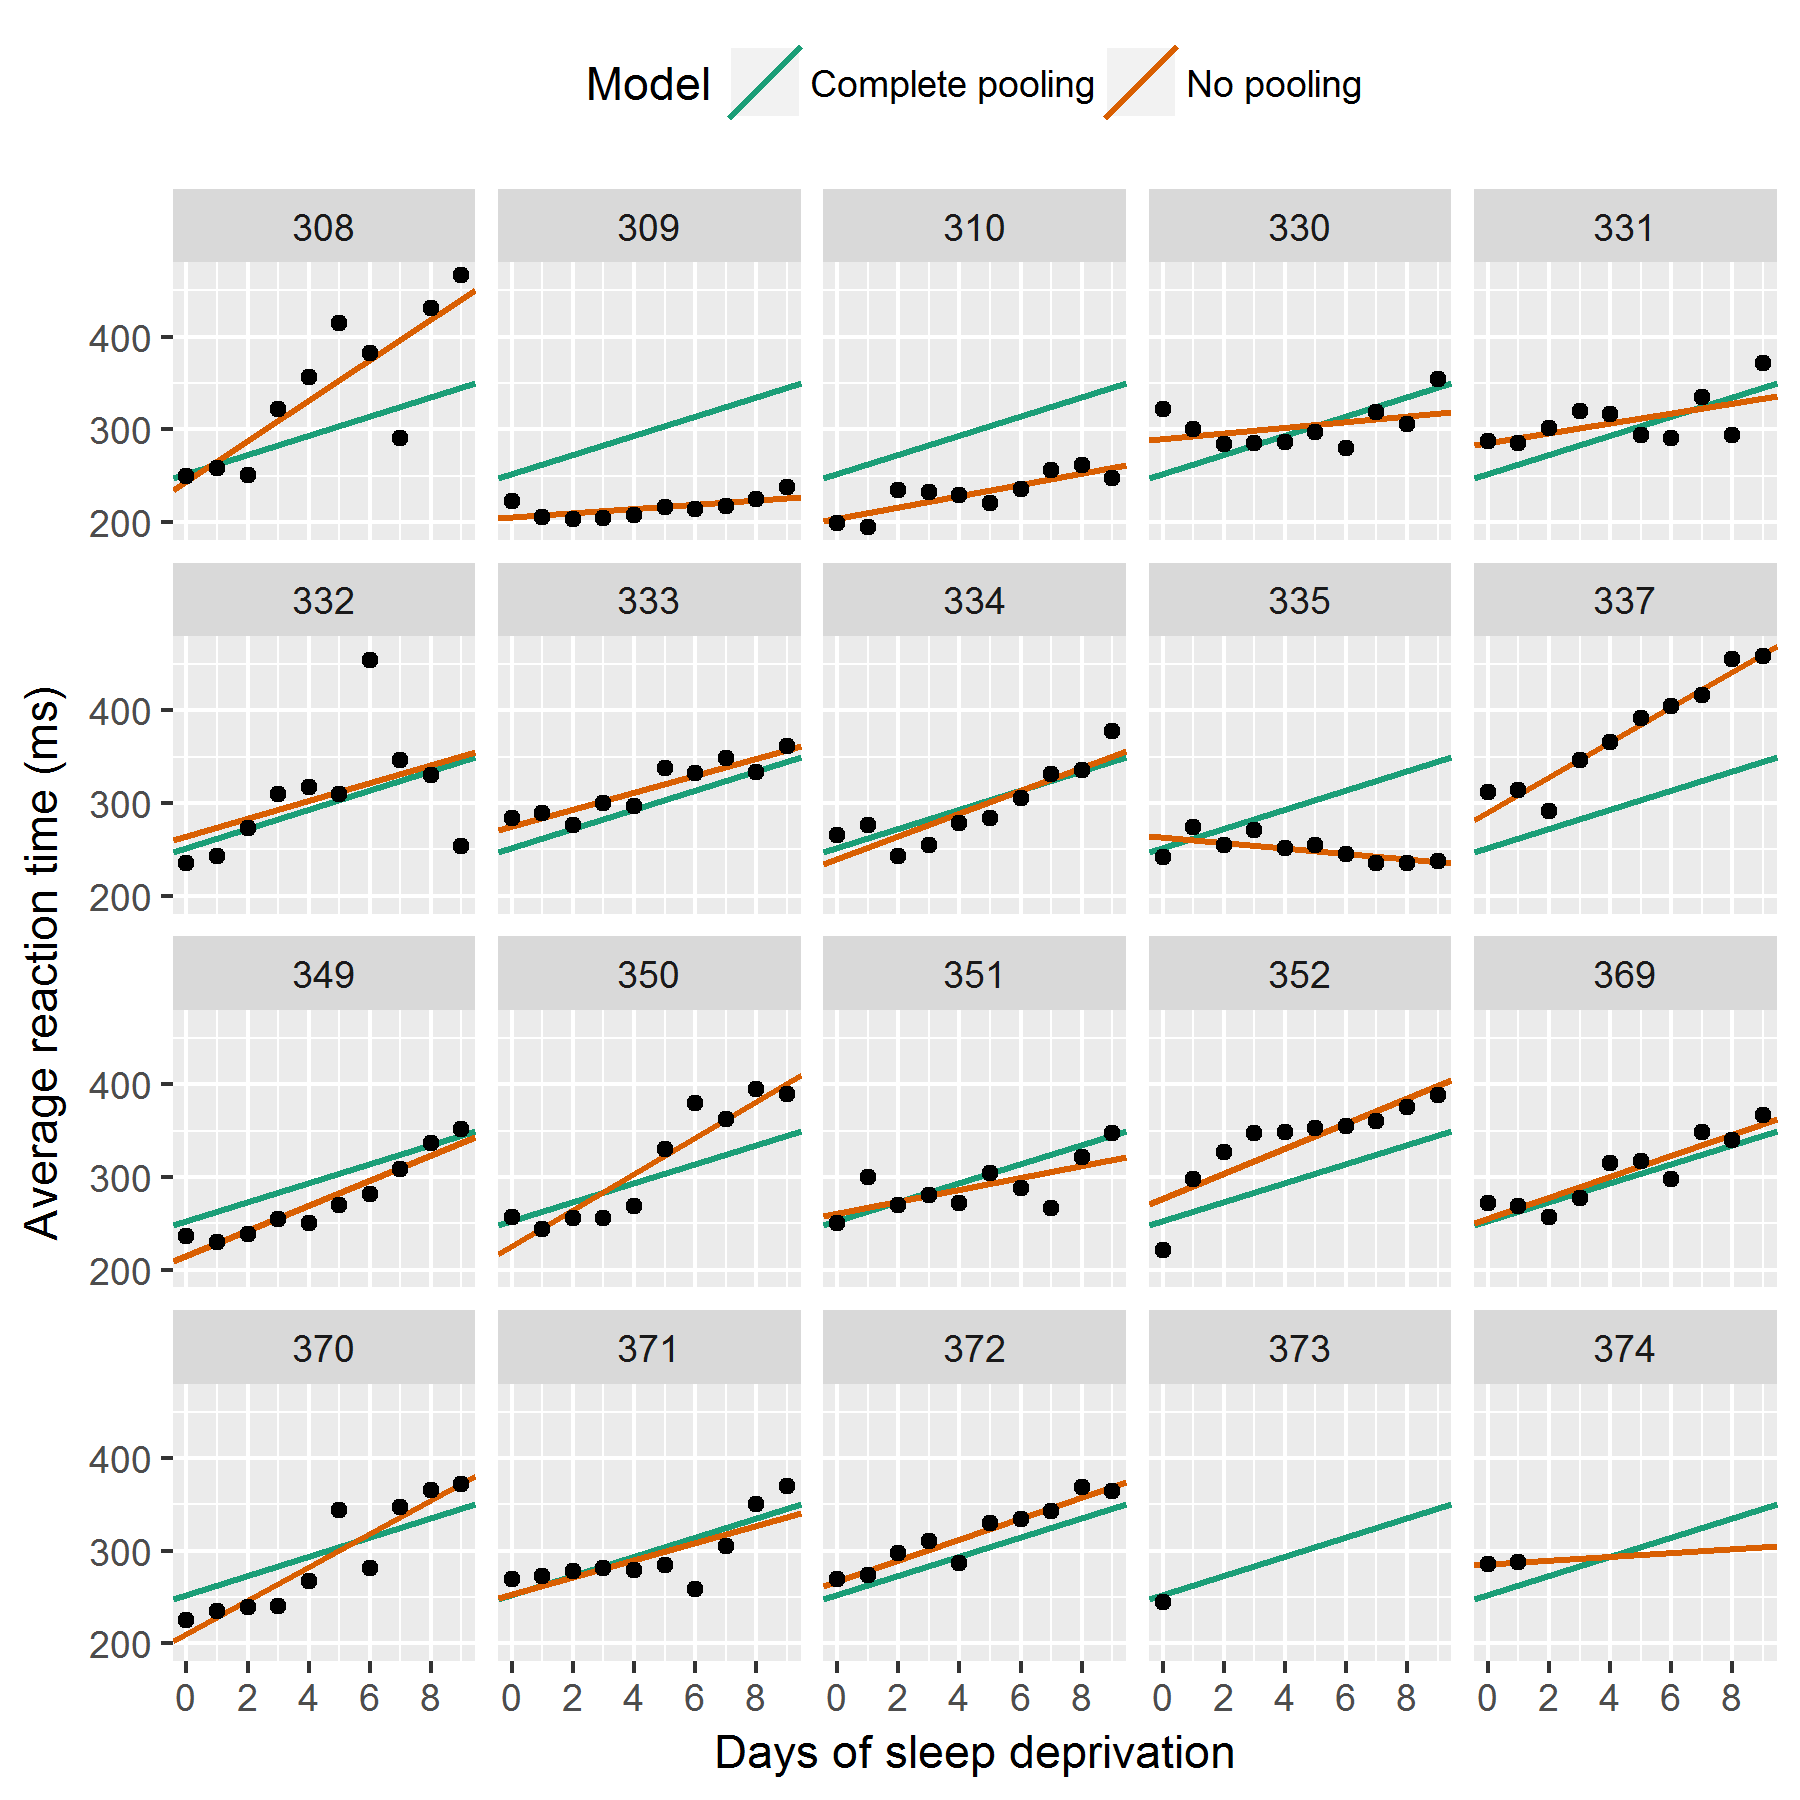
\includegraphics[width=0.6\textwidth]{lectures/day_5_theory_of_mems/figures/pooling-vs-no-pooling-1.png}
\end{frame}

\begin{frame}
    \textbf{Partial pooling} using a Mixed Effects Model
    \centering
    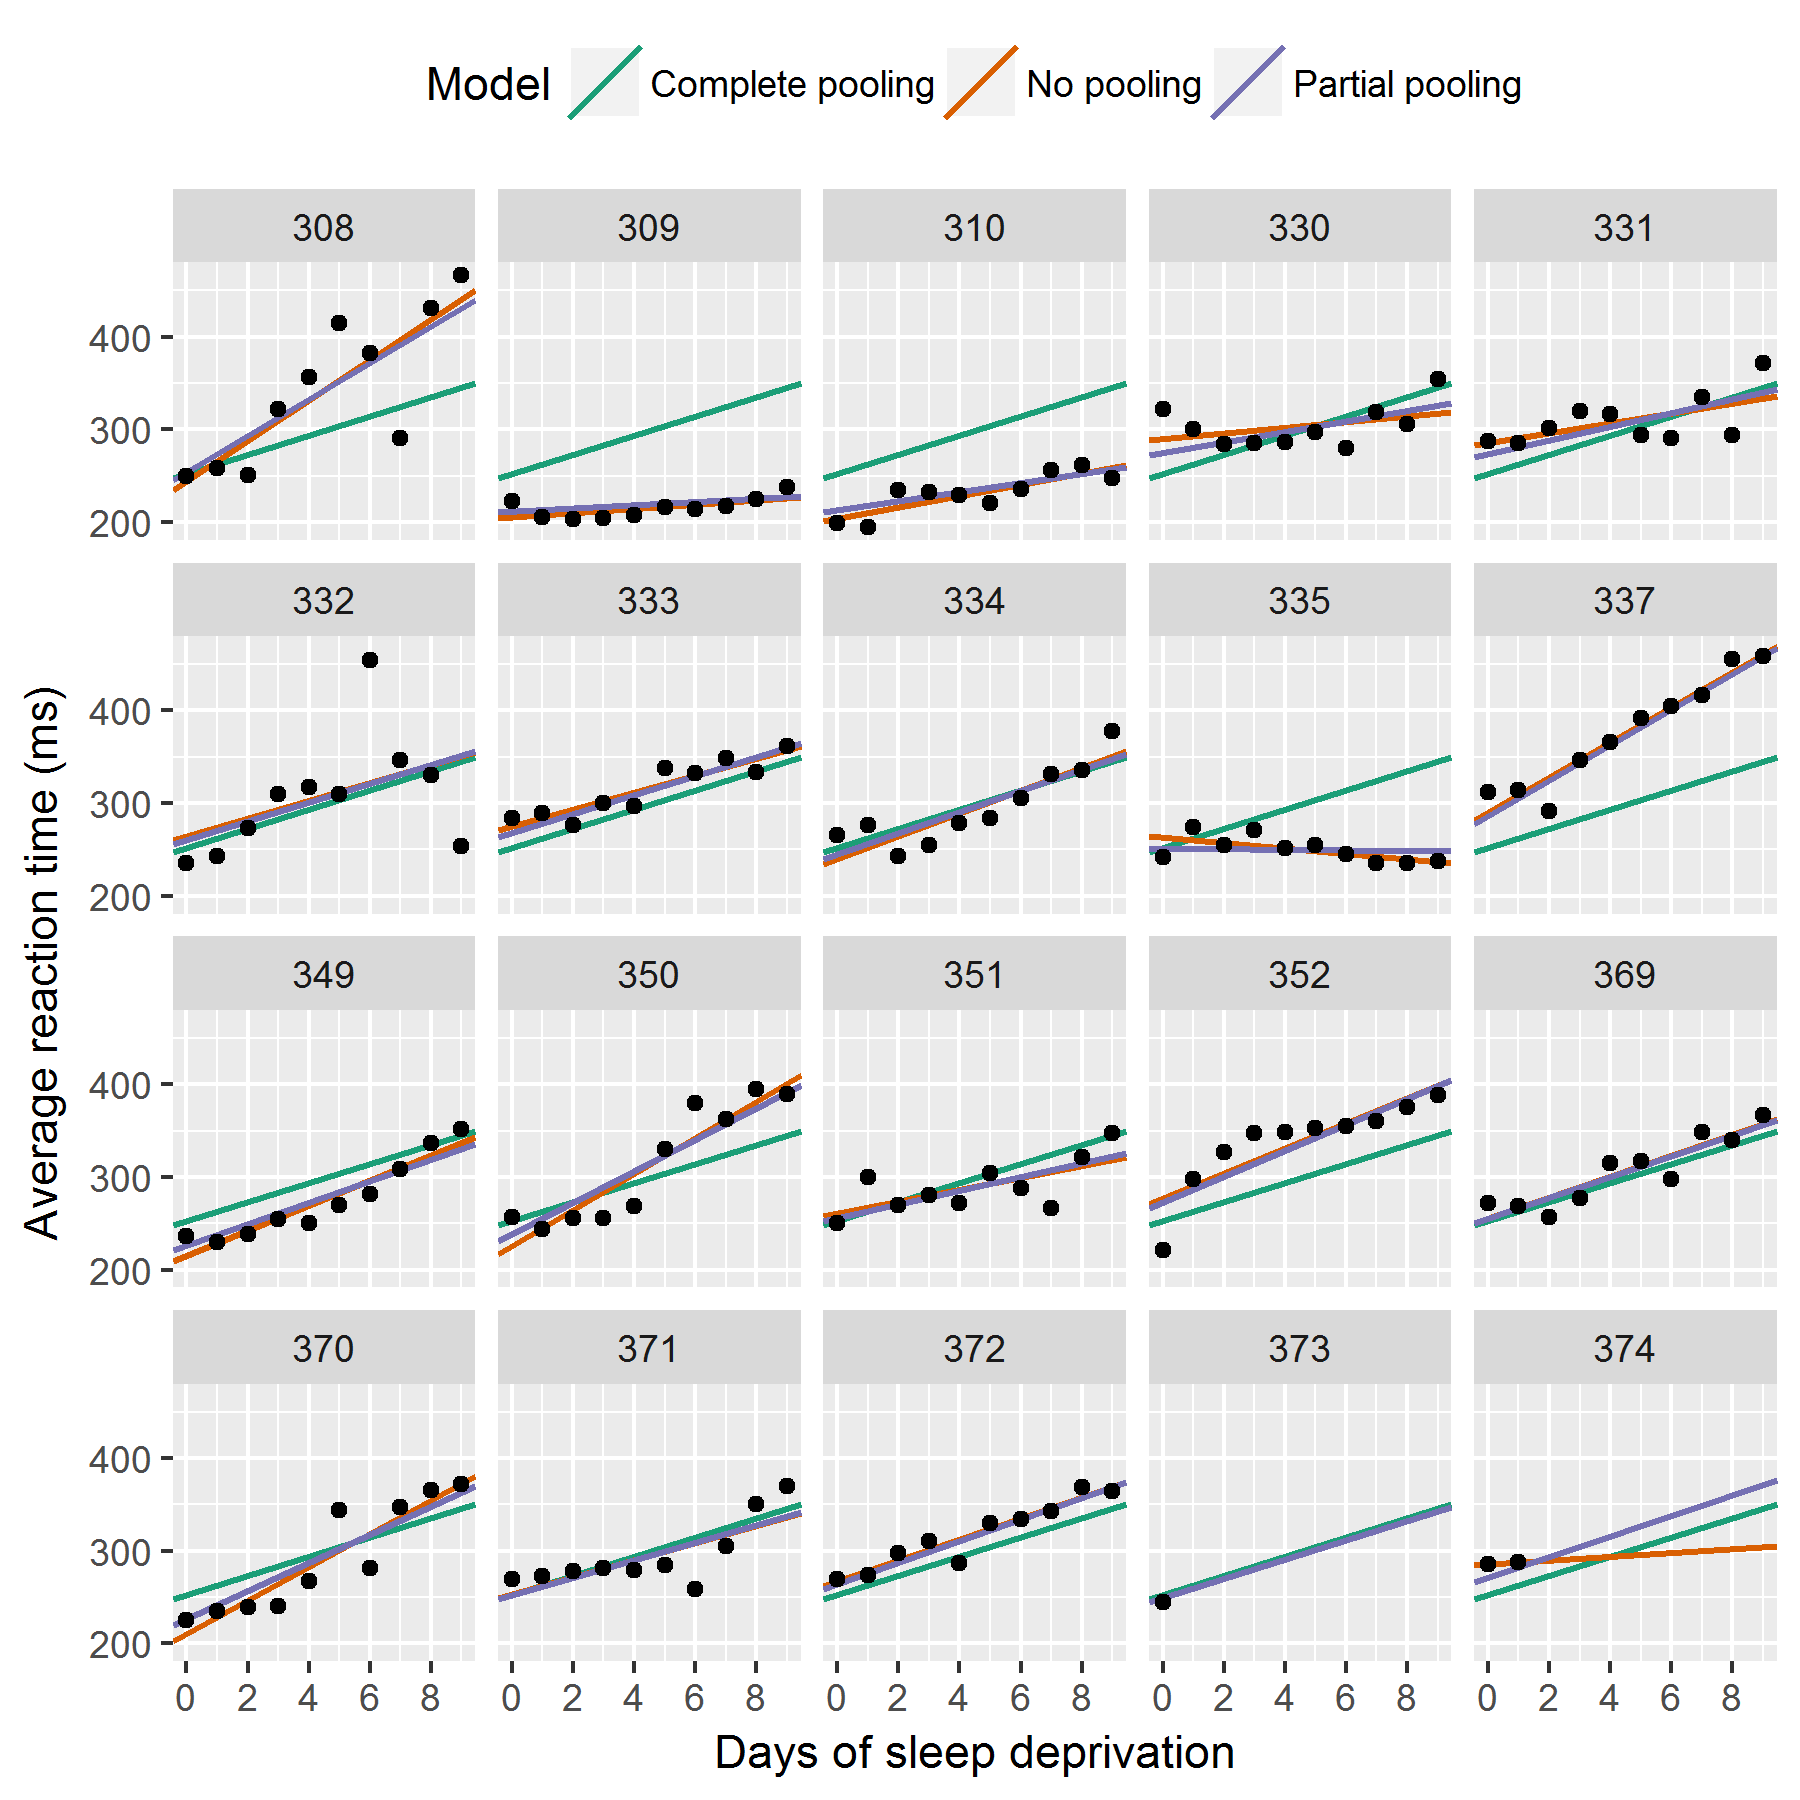
\includegraphics[width=0.6\textwidth]{lectures/day_5_theory_of_mems/figures/partial-pooling-vs-others-1.png}

    \textbf{No pooling} and \textbf{partial pooling} lines are mostly equal. When they differ, it’s because the partial pooling line is pulled slightly towards the \textbf{complete pooling} line.
    
\end{frame}

\begin{frame}
    Which \textbf{shrinks} estimated parameters towards the underlying population average

    \begin{center}
          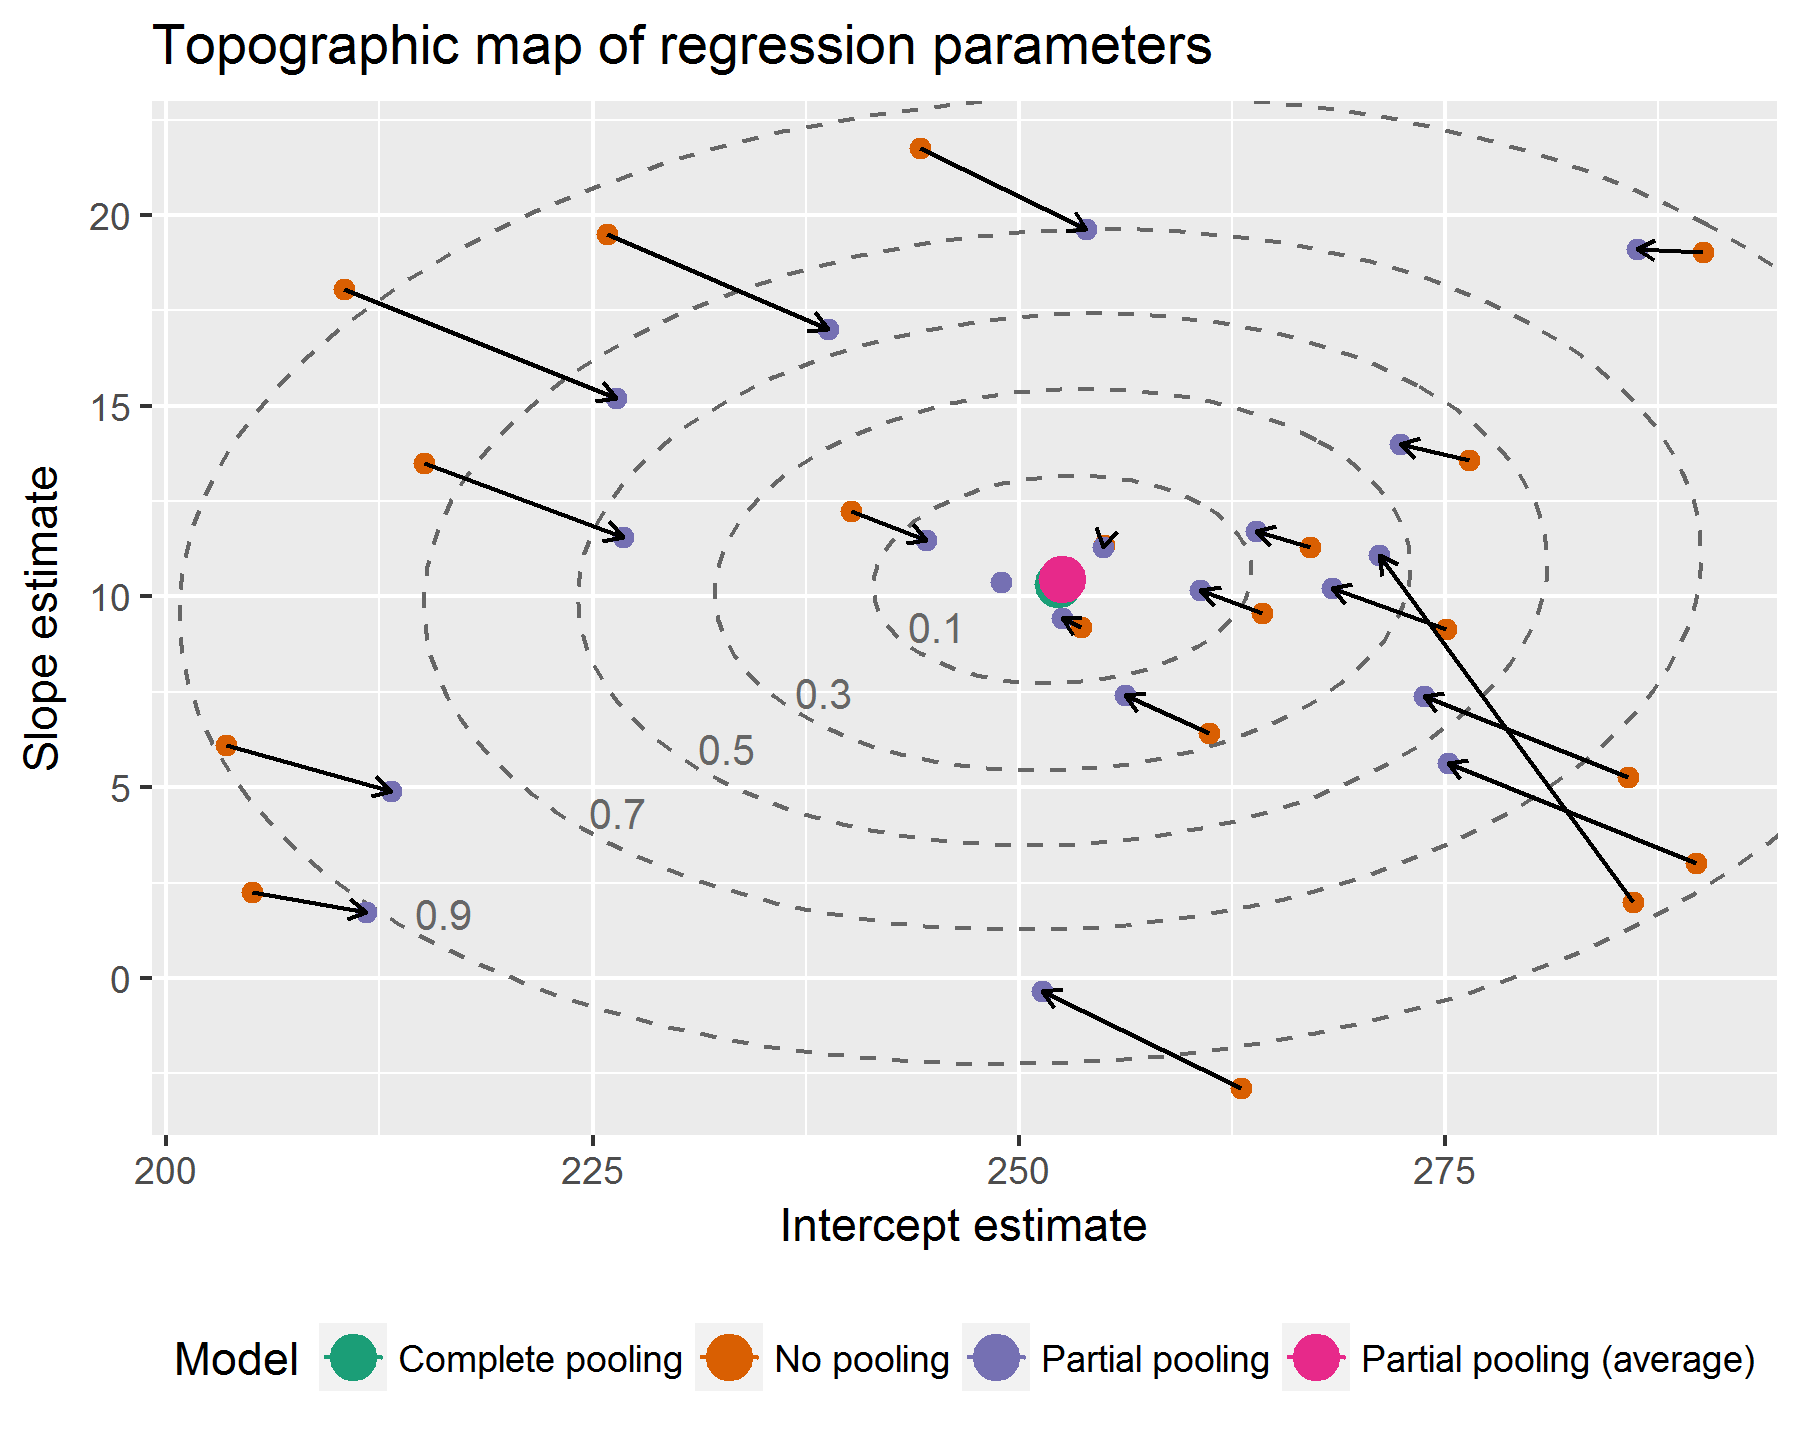
\includegraphics[width=0.6\textwidth]{lectures/day_5_theory_of_mems/figures/topographic-map-3-1.png}  
    \end{center}

\end{frame}

% Slide 20: Recapitulation of Day 5
\begin{frame}{Recapitulation - Week 5}
\large
By the end of today, you should understand:
\begin{itemize}
  \item How a \textbf{Mixed Effects Model} is expressed as \textbf{formula} and in \textbf{matrix notation}.
  \item What the various \textbf{stochastic part matrices} in LMM are.
  \item The \textbf{assumptions} of Linear Mixed Effects Models.
  \item The difference between \textbf{Random Intercept} and \textbf{Random Slope} models.
  \item The terms \textbf{Nested} and \textbf{Crossed} Random Effects.
  \item How to obtain unbiased \textbf{REML} estimates for the variance components.
  \item The concepts of \textbf{Pooling} and \textbf{BLUPs}.
\end{itemize}
\end{frame}

\end{document}